
\section{ESTO ES PARA QUITAR, DEJO AQUÍ TODO LO QUE HEMOS IDO APUNTANDO}



\begin{description}


\item[* MR4. More resources:] Si es satisfactible y aumentamos los recursos  (hay más obreros) $\rightarrow$  el resultado tiene que ser satisfactible y el makespan se reduce o se queda igual ($<=$).

\item[MR5. Fewer resources:] Si es satisfactible y disminuimos los recursos  (hay menos obreros)  $\rightarrow$  el resultado tiene que ser uno de estos dos casos: 

\begin{itemize}
    \item Satisfactible y el makespan se amplía o se queda igual ($>=$)
    \item o es insatisfactible  (porque no cumple  forall( r in RESOURCE, t in TASK) ( res[r,t]  $<=$ L[r])).
\end{itemize}





\item[MR6. Deleted precedence:]  Si es satisfactible y quitamos una restricción de precedencia $\rightarrow$ el resultado tiene que ser satisfactible y además el makespan se reduce o se queda igual ($<=$).




\item [MR7. Added precedences:] Si es satisfactible y se añade una precedencia que no forme ciclos $\rightarrow$ el resultado tiene que ser uno de estos dos casos: 

\begin{itemize}
    \item Satisfactible y el makespan se amplía o se queda igual ($>=$)
    \item o es insatisfactible  ¿esto no es otra forma de decir \textbf{Sequentiality of all tasks}?. Pensar que esto es añadir una restricción de precedencia y Sequentiality of all tasks necesita que todas las restricciones estén alineadas.
\end{itemize}



\item[MR8. Task time reduction:]  Si es satisfactible y reducimos las duraciones $\rightarrow$ el resultado tiene que ser satisfactible y el makespan se reduce o se queda igual ($<=$).

\item[MR9. Task time extension:]   Si es satisfactible y aumentamos las duraciones $\rightarrow$  el resultado tiene que ser satisfactible y el makespan se amplía o se queda igual ($>=$). 

Esto es debido a que el tiempo total es = sum(duration).


\item[MR10. Fewer overlapping tasks:]  Si es satisfactible y eliminamos un elemento del conjunto de tareas que no se solapan  $\rightarrow$ el resultado tiene que ser satisfactible y el makespan se reduce o se queda igual ($<=$).

\item[MR11. More overlapping tasks:]   Si es satisfactible y añadimos un elemento del conjunto de tareas que no se solapan  $\rightarrow$ el resultado tiene que ser uno de estos dos casos: 

\begin{itemize}
    \item Satisfactible y el makespan se amplía o se queda igual ($>=$)
    \item o es insatisfactible.
\end{itemize}

\item[MR12. Elements swapping: ] Si intercambiarmos las duraciones junto a   recursos requeridos por sus correspondientes tareas, entonces el makespan tiene que quedar igual.

\end{description}



\begin{table*}[t]
\begin{center}
\begin{tabular}{|c|p{3cm}|p{5cm}|p{5cm}|}
\hline
     & Basic & jobshop & moving \\
\hline
\hline
     \multicolumn{4}{|c|}{Donde aparece un asterisco significa que hay un mutante que mata a esa MR} \\
\hline
\hline

MR1 & * (Fig. \ref{Fig:RM-Sequentility-all-tasks}) basic-MUT-$\leq$-$<$  & NA. La matriz de datos obliga a que todas las tareas se ejecuten con precedencias & NA.  $\nexists$ precedence constraints  \\
     \hline
MR2  & * (Fig. \ref{Fig:Add-inverse-precedence}) basic-MUT-forall-exists    & NA. La matriz de datos obliga a que todas las tareas se ejecuten con precedencias & NA.  $\nexists$ precedence constraints\\
     \hline
MR3  &   & * (Fig. \ref{Fig:jobshop-forall-exists-1}) jobshopMUT-forall-exists-1   & \\
     &   & * (Fig. \ref{Fig:jobshop-forall-exists-2}) jobshopMUT-forall-exists-2   & \\
     &   & * (Fig. \ref{Fig:jobshop-y-o}) jobshopMUT-and-or  &   \\
          \hline
MR4   & & & (Fig. \ref{fig:more-trolleys}) no saca nada \\
  & NA. No trata recursos & NA. No trata recursos  &  (Fig. \ref{Fig:moving-con-mas-handlers}) En la versión 2.6.4 no se saca nada  pero hemos detectado que en la versión 2.5.5 hay un bug  \\
     \hline
MR5 & NA. No trata recursos & NA. No trata recursos  & NA. no se saca nada si deshechamos lo sucio \\
     \hline
\end{tabular}
\caption{NA means not available (no disponible) or
not applicable (no corresponde en el caso).}
\end{center}
\end{table*}


\newpage








A continuación, se decriben las Relaciones Metamórficas que se han encontrado para los tres tipos de problemas de schedule descritos. Estas relaciones permiten generar nuevos casos de prueba. 
Para validar cada Relación Metamórfica se ha tratado de encontrar la aplicación de un operador de mutación, que obtenga una versión mutada del progama MiniZinc, que se pueda matar con el caso de prueba siguiente obtenido con dicha relación Metamórfica.
Los operadores de mutación aplicados son algunos de los definidos en~\cite{puig2010equivalencias}. 
% puig2010equivalencias

%Relaciones metamórficas:

\begin{framed}
\textbf{MR1. Sequentiality of all tasks:} Si es satisfactible y se establecen precedencias de tal forma que todas las tareas se ejecutan en orden secuencial $\rightarrow$ el resultado tiene que ser satisfactible.
\end{framed}


\begin{figure*}[!h]
\begin{center}
\begin{minipage}{0.47\linewidth}
\begin{tikzpicture}

 \node [mynode](I) at (-1.5,1) {I (basic.dzn) };
 \node [mynode](O) at (-1.5,-2) {O (makespan 85)};
 \node [mylabel](code) at (0,-1) {basic.mzn};
 \node [mynode](I') at (1.5,1) {I' (basic-all-prec)};
 \node [mynode](O') at (1.5,-2) {O' (makespan 165)};

 \draw[myarrow](I) -- (O);
 \draw[myarrow](I') -- (O');

% \node [mynode,below= -0.3cm of I] (Icaption) {};
% \node [mynode,below= -0.3cm of I'] (I'caption) {};

\end{tikzpicture}
\subcaption{MR execution}
\end{minipage}
\begin{minipage}{0.05\linewidth}
\end{minipage}
\begin{minipage}{0.47\linewidth}
\begin{tikzpicture}

 \node [mynode](I) at (-1.5,1) {I (basic.dzn) };
 \node [mynode](O) at (-1.5,-2) {O (makespan 89)};
 \node [mylabel](code) at (0,-1) {\texttt{basicMUT<.mzn}};
 \node [mynode](I') at (1.5,1) {I' (basic-all-prec)};
 \node [mynodeRed](O') at (1.5,-2) {O' (UNSAT)};

 \draw[myarrow](I) -- (O);
 \draw[myarrow](I') -- (O');

% \node [mynode,below= -0.3cm of I] (Icaption) {d[0,0] = 1};
% \node [mynode,below= -0.3cm of I'] (I'caption) {d[0,0] = 100};

\end{tikzpicture}
\subcaption{Mutation execution}
\end{minipage}
\end{center}
\caption{MR1. En basic-all-prec están todas las precedencias secuenciales}
\label{Fig:RM-Sequentility-all-tasks}
\end{figure*}


\begin{framed}
\textbf{MR2. Add inverse precedence}

%Change forall to exists
Si es satisfactible y se añade una precedencia que es la inversa de una que ya existe (forma un cliclo) $\rightarrow$ es insatisfactible.
\end{framed}

\begin{framed}
\begin{center}
$MR2(i_1,i_2,o_1,o_2)$

$ \Updownarrow_{def}$

$Sat (O_1)) \wedge pre = pre \texttt{++} [pre[1,2], pre[1,1]]$  

$\Downarrow$

$Insat(O_2)$
\end{center}
\end{framed}



Si se añade una precedencia que es la inversa de una que ya existe entonces quiere decir que hay un ciclo. Pero, si al añadir esa precedencia inversa sigue dando solución y no es insat, entonces quiere decir que se ha puesto un exists en vez de un forall.

Obser: El que es insatisfactible tiene un forall y el que tiene solución tiene un exists es el programa mutado (basic-MUTexists)
En este caso, no se ha encontrado un operador definido para este cambio de cuantificadores
Podemos definirlo, indicando que se cambia un cuantificador lógico por otro (Existencial por universal o viceversa) .


Esto se hace para matar al mutante que cambia forall por exists.



Ejemplo correspondiente con el código \texttt{Codes/basic.mzn}
y con los datos
\texttt{Codes/basic.dzn} y a la Figura \ref{Fig:Add-inverse-precedence}







Original: constraint forall(i in PREC)

Cambiado: constraint exists(i in PREC)

En los datos se añade la precedencia  SOLDIERS $\rightarrow$ FUNDS para que forme  ciclo con la precedencia que ya existe que es
 FUNDS $\rightarrow$ SOLDIERS
   
   



\begin{figure*}[!h]
\begin{center}
\begin{minipage}{0.47\linewidth}
\begin{tikzpicture}

 \node [mynode](I) at (-1.5,1) {I (basic.dzn) };
 \node [mynode](O) at (-1.5,-2) {O (makespan = 85)};
 \node [mylabel](code) at (0,-1) {basic.mzn};
 \node [mynode](I') at (1.5,1) {I' (basic-cycle)};
 \node [mynode](O') at (1.5,-2) {O' (UNSAT)};

 \draw[myarrow](I) -- (O);
 \draw[myarrow](I') -- (O');

\end{tikzpicture}
\subcaption{Source test case - Al tener un ciclo es insatisfactible y esto es correcto}
\end{minipage}
\begin{minipage}{0.05\linewidth}
\end{minipage}
\begin{minipage}{0.47\linewidth}
\begin{tikzpicture}

 \node [mynode](I) at (-1.5,1) {I (basic.dzn) };
 \node [mynode](O) at (-1.5,-2) {O (makespan = 25 )};
 \node [mylabel](code) at (-1,-1) {\verb+basic-MUT-forall-exists.mzn+};
 \node [mynode](I') at (1.5,1) {I' (basic-cycle)};
 \node [mynodeRed](O') at (1.5,-2) {O' (end = 25)};

 \draw[myarrow](I) -- (O);
 \draw[myarrow](I') -- (O');

\end{tikzpicture}
\subcaption{Follow-up test case - Se puede matar al mutante basic-MUTexists.mzn}
\end{minipage}
\caption{MR2: se añade una precedencia que forme un ciclo en el grafo}
\label{Fig:Add-inverse-precedence}
\end{center}
\end{figure*}



\subsection{Schedule for Jobshop problem}

The job shop scheduling model given in Listing 2.2.10 gives a realistic example of the use of this disjunctive modelling capability. In job shop scheduling we have a set of jobs, each consisting of a sequence of tasks on separate machines: so task [i,j] is the task in the ith job performed on the jth machine. Each sequence of tasks must be completed in order, and no two tasks on the same machine can overlap in time. 

%\lstinputlisting[float=*, label=jobshopmzn,caption= jobshop.mzn code,language=Python,frame=single]{Codes/jobshop.mzn}

%\lstinputlisting[label=jobshopdzn,caption= mojobshop.dzn data,language=Python,frame=single]{Codes/jdata.dzn}

Trabajamos con \texttt{Codes/jobshop.mzn} y \texttt{Codes/jobshop.dzn}. Corresponde a la Figura \ref{Fig:jobshop-forall-exists-1}.


\begin{framed}
    \textbf{MR3. Extreme duration}
    
    Si es satisfactible y se amplía una duración, pongamos la primera  d[1] + $c$, donde $c >= sum(d[i,j]) \ \forall i$ and $\forall j$ 
    entonces el makespan de O' debe ser mayor estricto que el makespan O.
\end{framed}


\begin{framed}
\begin{center}
$MR3(i_1,i_2,o_1,o_2)$

$ \Updownarrow_{def}$

$Sat (O_1)) \wedge d2[1] =  d1[0,0] + c$, where $c >= sum(d1[i,j]) \ \forall i$ and $\forall j$  

$\Downarrow$

$Sat(O_2) \wedge  \texttt{makespan($O_2$)} > \texttt{makespan($O_1$)} $
\end{center}
\end{framed}


Hacemos un mutante donde cambiamos un \texttt{forall} por \texttt{exists}, 

\texttt{jobshopMUT-forall-exists-1.mzn}.

En este caso se aplica el nuevo operador de mutación en el que cambiamos un cuantificador por otro 
y este cambio se puede hacer en otras partes del código dando lugar a nuevos mutantes.

\begin{figure*}[h]
\begin{minipage}{0.49\linewidth}
\begin{center}
\begin{tikzpicture}

 \node [mynode](I) at (-2,1) {I (jdata.dzn) };
 \node [mynode](O) at (-2,-2) {O (end = 30)};
 \node [mylabel](code) at (0,-1) {jobshop.mzn};
 \node [mynode](I') at (2,1) {I' (jdata+d)};
 \node [mynode](O') at (2,-2) {O' (end = 126)};

 \draw[myarrow](I) -- (O);
 \draw[myarrow](I') -- (O');

 \node [mynode,below= -0.3cm of I] (Icaption) {d[0,0] = 1};
 \node [mynode,below= -0.3cm of I'] (I'caption) {d[0,0] = 100};

\end{tikzpicture}
\subcaption{MR execution}
\label{Fig: MR3. jobshop-forall-exists-1-b}
\end{center}
\end{minipage}
\begin{minipage}{0.49\linewidth}
\begin{center}
\begin{tikzpicture}

 \node [mynode](I) at (-2,1) {I (jdata.dzn) };
 \node [mynode](O) at (-2,-2) {O (end = 15)};
 \node [mylabel](code) at (-1,0) {jobshopMUT-forall-exists-1.mzn};
 \node [mynode](I') at (2,1) {I' (jdata+d)};
 \node [mynodeRed](O') at (2,-2) {O' (end = 15)};

 \draw[myarrow](I) -- (O);
 \draw[myarrow](I') -- (O');

 \node [mynode,below= -0.3cm of I] (Icaption) {d[0,0] = 1};
 \node [mynode,below= -0.3cm of I'] (I'caption) {d[0,0] = 100};

\end{tikzpicture}
\subcaption{Mutation execution}
\label{Fig: MR3. jobshop-forall-exists-1-a}
\end{center}
\end{minipage}
\caption{MR3. Caso 1 de cambio forall - exists en el código de jobshop}
\label{Fig: MR3. jobshop-forall-exists-1}
\end{figure*}









\begin{figure*}[h]
\begin{minipage}{0.49\linewidth}
\begin{center}
\begin{tikzpicture}

 \node [mynode](I) at (-2,1) {I (jdata.dzn) };
 \node [mynode](O) at (-2,-2) {O (end = 30)};
 \node [mylabel](code) at (0,-1) {jobshop.mzn};
 \node [mynode](I') at (2,1) {I' (jdata+d)};
 \node [mynode](O') at (2,-2) {O' (end = 126)};

 \draw[myarrow](I) -- (O);
 \draw[myarrow](I') -- (O');

 \node [mynode,below= -0.3cm of I] (Icaption) {d[0,0] = 1};
 \node [mynode,below= -0.3cm of I'] (I'caption) {d[0,0] = 100};

\end{tikzpicture}
\subcaption{MR execution}
\end{center}
\end{minipage}
\begin{minipage}{0.49\linewidth}
\begin{center}
\begin{tikzpicture}

 \node [mynode](I) at (-2,1) {I (jdata.dzn) };
 \node [mynode](O) at (-2,-2) {O (end = 21)};
 \node [mylabel](code) at (-1,-1) {\verb+jobshopMUT-forall-exists-2.mzn+};
 \node [mynode](I') at (2,1) {I' (jdata+d)};
 \node [mynodeRed](O') at (2,-2) {O' (end = 21)};

 \draw[myarrow](I) -- (O);
 \draw[myarrow](I') -- (O');

 \node [mynode,below= -0.3cm of I] (Icaption) {d[0,0] = 1};
 \node [mynode,below= -0.3cm of I'] (I'caption) {d[0,0] = 100};

\end{tikzpicture}
\subcaption{Mutation execution}
\end{center}
\end{minipage}
\caption{MR3. Caso 2 de cambio forall - exists en el código de jobshop}
\label{Fig:jobshop-forall-exists-2}
\end{figure*}









La Metamorphic Relation \texttt{Extreme Durations}, también mata a otro mutante. 

\texttt{jobshopMUT-and-or.mzn}

En este caso se ha cambiado la conjunción por la disyunción: \verb+/\  -> \/+ 


\begin{figure*}[h]
\begin{minipage}{0.49\linewidth}
\begin{center}
\begin{tikzpicture}

 \node [mynode](I) at (-2,1) {I (jdata.dzn) };
 \node [mynode](O) at (-2,-2) {O (end = 30)};
 \node [mylabel](code) at (0,-1) {jobshop.mzn};
 \node [mynode](I') at (2,1) {I' (jdata+d)};
 \node [mynode](O') at (2,-2) {O' (end = 126)};

 \draw[myarrow](I) -- (O);
 \draw[myarrow](I') -- (O');

 \node [mynode,below= -0.3cm of I] (Icaption) {d[0,0] = 1};
 \node [mynode,below= -0.3cm of I'] (I'caption) {d[0,0] = 100};

\end{tikzpicture}
\subcaption{MR execution}
\end{center}
\end{minipage}
\begin{minipage}{0.49\linewidth}
\begin{center}
\begin{tikzpicture}

 \node [mynode](I) at (-2,1) {I (jdata.dzn) };
 \node [mynode](O) at (-2,-2) {O (end = 0)};
 \node [mylabel](code) at (-0.7,-1) {jobshopMUT-and-or.mzn};
 \node [mynode](I') at (2,1) {I' (jdata+d)};
 \node [mynodeRed](O') at (2,-2) {O' (end = 0)};

 \draw[myarrow](I) -- (O);
 \draw[myarrow](I') -- (O');

 \node [mynode,below= -0.3cm of I] (Icaption) {d[0,0] = 1};
 \node [mynode,below= -0.3cm of I'] (I'caption) {d[0,0] = 100};

\end{tikzpicture}
\subcaption{Mutation execution}
\end{center}
\end{minipage}
\caption{MR3. jobshop cambiar y por o}
\label{Fig:jobshop-y-o}
\end{figure*}




\subsection{cumulative constraint (resources)}


The cumulative constraint is used for describing cumulative resource usage.

\texttt{cumulative(array[int] of var int: s, array[int] of var int: d, array[int] of var int: r, var int: b)}

Schedule for moving furniture:
It requires that a set of tasks given by start times $s$, durations $d$, and resource requirements $r$, never require more than a global resource bound $b$ at any one time.

Los códigos son \texttt{Codes/moving.mzn} y \texttt{Codes/moving.dzn}.

%\lstinputlisting[label=movingmzn,caption= moving.mzn code,language=Python,frame=single]{Codes/moving.mzn}

%\lstinputlisting[label=movingdzn,caption= moving.dzn data,language=Python,frame=single]{Codes/moving.dzn}


%\begin{figure*}[h]
%    \centering
    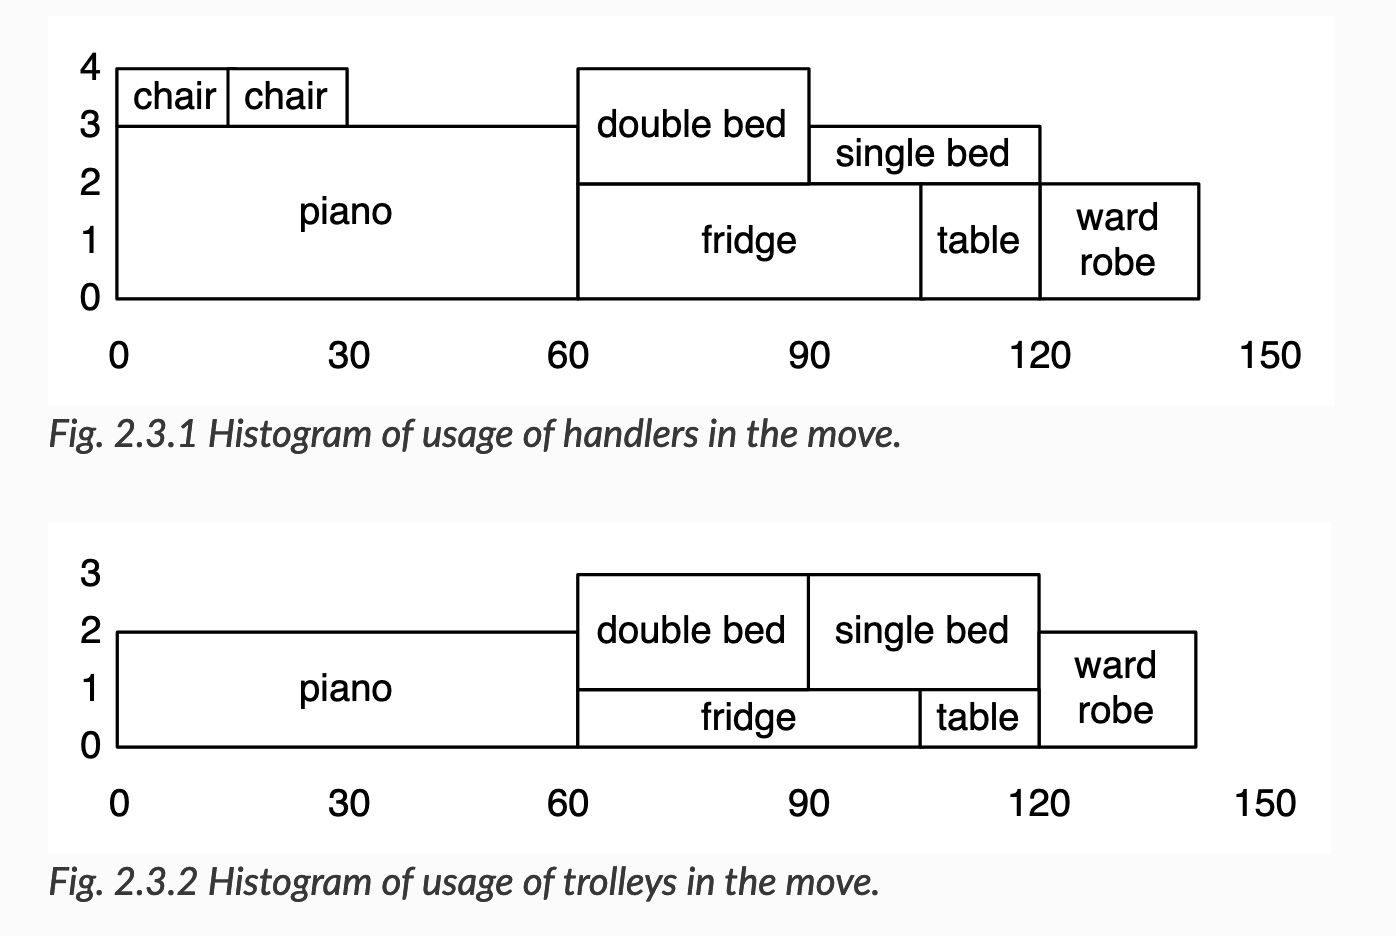
\includegraphics[width=0.5\textwidth]{Figures/movingFurniture.jpg}
%    \caption{Moving furniture for moving.dzn data}
%    \label{fig:mesh1}
%\end{figure*}











Las Relaciones metamórficas (MRs) para moving son 

%\begin{description}
\begin{framed}
    \textbf{MR4. More resources} 
    
    Si es satisfactible y aumentamos los recursos  (handlers and trolleys) $\rightarrow$  el resultado tiene que ser satisfactible y el makespan (end) se reduce o se queda igual ($<=$).
\end{framed}

$ i_1 = (T1, D1, - , - , R1 , time1 )$

$ i_2 = (T2, D2, - , - , R2 , time2 )$

where 
$R1 = [(l1_1,up1_1), \dots, (l1_k,up1_k)]$

$O_1 = S(i_1)$ 
 
\begin{framed}
\begin{center}
$MR4(i_1,i_2,o_1,o_2)$

$ \Updownarrow_{def}$

$Sat (O_1)) \wedge$ 

$\forall i \in \{1,\dots,k\} \ \exists j \in \{1,\dots,k\}$ and $\exists c >0$ \texttt{such as} $up2_j = up1_j + c $  

$\Downarrow$

$Sat(O_2) \wedge  \texttt{makespan($O_2$)} =< \texttt{makespan($O_1$)} $
\end{center}
\end{framed}



\begin{itemize}
    \item[(1)] En \textbf{moving-more-available-trolleys.dzn} cambio respecto al original \textbf{moving.dzn}:
    la variable \texttt{available-trolleys}: 3 $\rightarrow$ 6.
\end{itemize}    

Generamos un mutante (movingMUTtrolleys.mzn) intercambiando dos parámetros de la restricción cumulative.

Original: constraint cumulative(start, duration, trolleys, available-trolleys);

Cambio: constraint cumulative(start, trolleys, duration, available-trolleys);
En este caso se ha aplicado el operador ISV definido en ~\cite{puig2010equivalencias}.

El resultado es NA. 
Pues con el mutante me salen los dos insatisfactibles y esto no me dice nada, ver Figura \ref{fig:more-trolleys} .

\begin{figure*}[h]
\begin{center}
\begin{minipage}{0.49\linewidth}
\begin{tikzpicture}

 \node [mynode](I) at (-1.5,1) {I (moving.dzn) };
 \node [mynode](O) at (-1.5,-2) {O (end = 140)};
 \node [mylabel](code) at (0,-1) {moving.mzn};
 \node [mynode](I') at (1.5,1) {I' (moving+trolleys.dzn)};
 \node [mynode](O') at (1.5,-2) {O' (end = 120)};

 \draw[myarrow](I) -- (O);
 \draw[myarrow](I') -- (O');

 \node [mynode,below= -0.3cm of I] (Icaption) {availableTrolleys: 3};
 \node [mynode,below= -0.3cm of I'] (I'caption) {availableTrolleys: 6};

\end{tikzpicture}
\subcaption{MR execution}
\end{minipage}
\begin{minipage}{0.49\linewidth}
\begin{tikzpicture}


 \node [mynode](I) at (-1.5,1) {I (moving.dzn)};
 \node [mynodeRed](O) at (-1.5,-2) {O (UNSAT)};
 \node [mylabel](code) at (0,-1) {movingMUT1.mzn};
 \node [mynode](I') at (1.5,1) {I' (moving+trolleys.dzn)};
 \node [mynodeRed](O') at (1.5,-2) {O' (UNSAT)};

 \draw[myarrow](I) -- (O);
 \draw[myarrow](I') -- (O');

 \node [mynode,below= -0.3cm of I] (Icaption) {availableTrolleys: 3};
 \node [mynode,below= -0.3cm of I'] (I'caption) {availableTrolleys: 6};

\end{tikzpicture}
\subcaption{Mutation execution}
\end{minipage}
\caption{MR4. EL CASO DE PRUEBA NUEVO NO SIRVE, PORQUE CON EL CASO ORIGINAL YA SE MATA a movingMUT1.mzn (es insatisfactible).}
\label{fig:more-trolleys}
\end{center}
\end{figure*}

\begin{itemize}
    \item[(2)] En \textbf{moving-more-available-handlers.dzn} cambio respecto al original \textbf{moving.dzn}:  la variable \texttt{availableHandlers}: 4 $\rightarrow$ 6.
\end{itemize}   
        
        No se reduce el makespan aunque lo pongamos la variable \texttt{availableHandlers} a 100 o a 100000. 
        Tener más pesonas para la mudanza no hace que se termine antes. Si que es cierto que si hay 3 personas entonces end = 170, pero a partir de 3 siempre es end = 140,... hasta el "infinito".
        
\medskip



        
        Genero un mutante (movingMUT1.mzn) intercambiando dos parámetros de la restricción cumulative.
        
Original: constraint cumulative(start, duration, handlers, availableHandlers);

Cambio: constraint cumulative(start, handlers, duration, availableHandlers);

La variable availableHandlers = 40;

        \begin{lstlisting}
        Running movingMUT1.mzn with moving.dzn
        start = [0, 3, 90, 60, 120, 6, 5, 48]
        end = 140
        
        Running moving-MUT1.mzn with moving-more-available-handlers.dzn
        =====UNSATISFIABLE=====
        \end{lstlisting}

\begin{framed}
I (moving.dzn) -- movingMUT1.mzn $\rightarrow$ O (end = 140)

I' (moving-more-available-trolleys.dzn) -- movingMUT1.mzn $\rightarrow$ O' (UNSAT)
\end{framed}    




En este caso sale UNSAT porque en movingMUT1.mzn he intercambiado en la restricciçon cumulative dos parámetros: handlers y duration. Estos reciben datos que no son semejantes, 

duration = [60, 45, 30, 30, 20, 15, 15, 15];

handlers = [3, 2, 2, 1, 2, 1, 1, 2];



Por otra parte en I' se ha aumentado el valor de la variable availableHandlers de 4 a 40; Entonces al tener más personal para la mudanza, el tiempo se debe quedar igual o reducir, pero NUNCA DEBE SER UNSAT. 
Es UNSAT porque al intercambiar duration y handlers, ahora se necesitan 60 personas para mover el piano y solo hay 40.
NO LO ENTIENDO, HAGO PRUEBAS Y VEO cuando la variable availableHandlers $\in [30, 59]$ es UNSAT para el resto de valores es satisfactible.

Realmente hemos comprobado que nuestra MT-regla no se cumple y podemos matar al MUTANTE movingMUT1.mzn

ESTE ERROR ESTÁ EN LA VERISÓN DE MINIZiNC

MiniZinc to FlatZinc converter, version 2.5.5, build 273041792
% mac mini
Copyright (C) 2014-2021 Monash University, NICTA, Data61

Lo he probado en la versión
Version 2.5.5 - 273051464 
% macBook air portátil
y ya funciona bien.



EN LA VERSIÓN ACTUAL YA ESTÁ ARREGLADO


\begin{figure*}[h]
\begin{minipage}{0.49\linewidth}
\begin{center}
\begin{tikzpicture}

 \node [mynode](I) at (-1.5,1) {I (moving.dzn) };
 \node [mynode](O) at (-1.5,-2) {O (end = 140)};
 \node [mylabel](code) at (0,-1) {moving.mzn};
 \node [mynode](I') at (1.5,1) {I' (moving+Handlers.dzn)};
 \node [mynode](O') at (1.5,-2) {O' (end = 140)};

 \draw[myarrow](I) -- (O);
 \draw[myarrow](I') -- (O');

 \node [mynode,below= -0.3cm of I] (Icaption) {availableHandlers: 4};
 \node [mynode,below= -0.3cm of I'] (I'caption) {availableHandlers: 40};

% \draw[->,red, thick](T1) -- (T2);
\end{tikzpicture}
\subcaption{MR execution}
\end{center}
\end{minipage}
\begin{minipage}{0.49\linewidth}
\begin{center}

\begin{tikzpicture}


 \node [mynode](I) at (-1.5,1) {I (moving.dzn)};
 \node [mynodeGreen](O) at (-1.5,-2) {O (end = 140)};
 \node [mylabel](code) at (0,-1) {movingMUT-handlers.mzn};
 \node [mynode](I') at (1.5,1) {I' (moving+Handlers.dzn)};
 \node [mynodeRed](O') at (1.5,-2) {O' (UNSAT)};

 \draw[myarrow](I) -- (O);
 \draw[myarrow](I') -- (O');

 \node [mynode,below= -0.3cm of I] (Icaption) {availableHandlers: 4};
 \node [mynode,below= -0.3cm of I'] (I'caption) {availableHandlers: 40};

% \draw[->,red, thick](T1) -- (T2);
\end{tikzpicture}
\subcaption{Mutation execution}
\end{center}
\end{minipage}
\caption{MR4. VERDE SIGNIFICA QUE ES RARO. ES DECIR, EN LA VERSIÓN 2.5.5 SALE end = 140 Y EN LA VERSIÓN 2.6.3 ES UNSATISFIABLE.
El rojo indica que se puede matar al Mutante movingMUT1.mzn}
\label{Fig:moving-con-mas-handlers}
\end{figure*}
%\end{description}

Es decir, el ejemplo bueno es ejecutar moving.mzn con la entrada I (moving.dzn) que tiene la variable  availableHandlers con el valor 4. Esta ejecución tiene como salida la variable end a 140. Cambiamos la entrada I' (moving-more-available-handlers.dzn) y ponemos la variable availableHandlers a 40. La ejecución con moving.mzn da una respueta de end = 140 correspondiente a O'.

Ahora ejecuto el caso que va mal. Es el mutante movingMUT-handlers.mzn. Con la entrada I (moving.dzn) que tiene la variable  availableHandlers a 4, tiene como salida la variable end a 140. Esto es raro, porque al intercambiar los parámetros de entrada, ya no tiene sentido y de hecho lo lógico es que salga Insatisfacble. Vemos que sale 140 en la versión 2.5.5, pero comprobamos otra versión de miniznc, la 2.6.3 y es UNSAT, vamos lo que debe ser.

\begin{comment}
\begin{figure*}
    \centering
    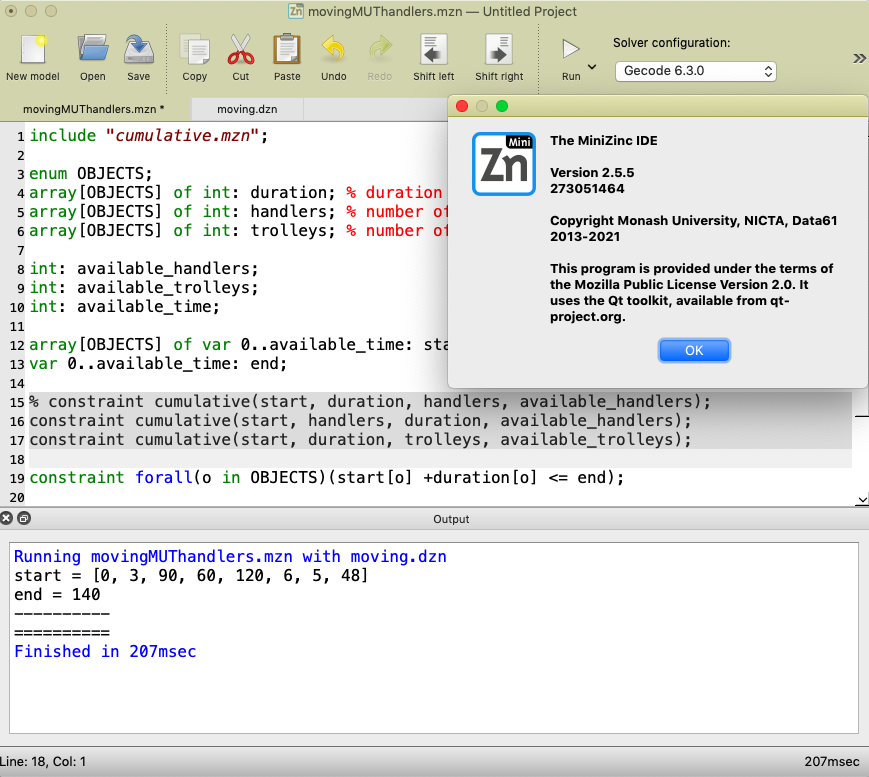
\includegraphics[scale = 0.3]{Figures/ScreenShot_minizinc_bug_1.png}
    \caption{SE VE MUY BORROSO}
    \label{fig:ScreenShot_minizinc_bug_1}
\end{figure*}

\begin{figure*}
    \centering
    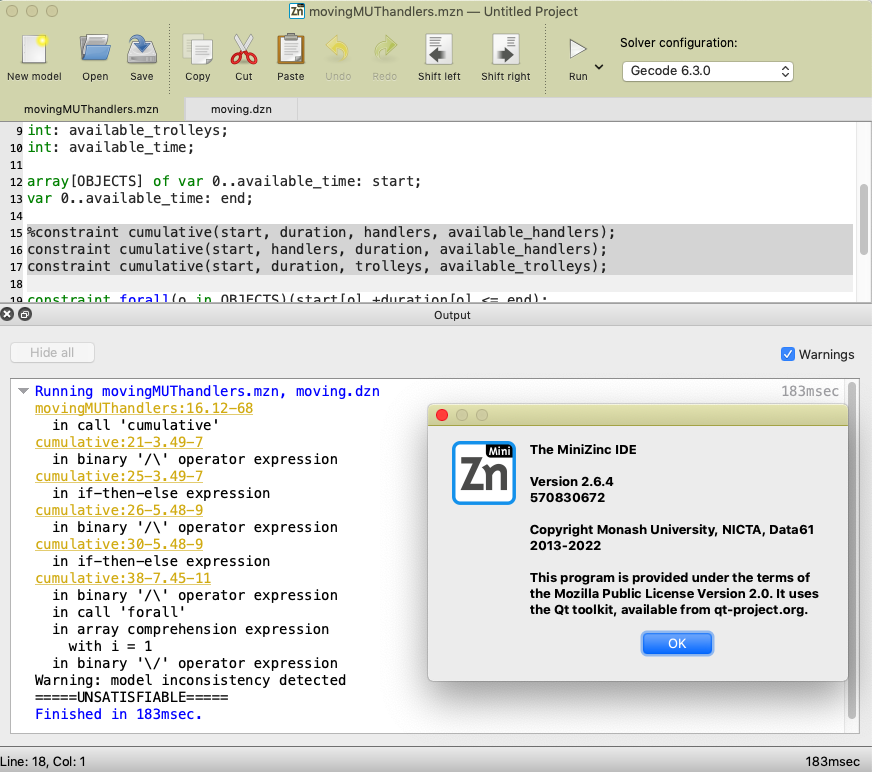
\includegraphics[scale = 0.3]{Figures/ScreenShot_minizinc_bug_2.png}
    \caption{SE VE MUY BORROSO}
    \label{fig:ScreenShot_minizinc_bug_2}
\end{figure*}
\end{comment}




\begin{framed}
    
\textbf{MR5. Fewer resources}

Si es satisfactible y disminuimos elos recursos  (handlers and trolleys)  $\rightarrow$  el resultado tiene que ser uno de estos dos casos: 
\begin{itemize}
    \item Satisfactible y el makespan se amplía o se queda igual (\texttt{>=})
    \item o es insatisfactible  
    %(porque no cumple  forall( r in RESOURCE, t in TASK) ( res[r,t]  $<=$ L[r])).
\end{itemize}
\end{framed}

\begin{framed}
\begin{center}
$MR5(i_1,i_2,o_1,o_2)$

$ \Updownarrow_{def}$

$Sat (O_1)) \wedge$ 

$\forall i \in \{1,\dots,k\} \ \exists j \in \{1,\dots,k\}$ and $\exists c >0$ \texttt{such as} $up2_j = up1_j - c $  

$\Downarrow$

$(InSat(O_2)) \vee $

$(Sat(O_2) \wedge \texttt{makespan($O_2$)} \geq \texttt{makespan($O_1$)}) $
\end{center}
\end{framed}





\begin{figure*}[h]
\begin{minipage}{0.49\linewidth}
\begin{center}
\begin{tikzpicture}

 \node [mynode](I) at (-1.5,1) {I (cumul-sched.dzn) };
 \node [mynode](O) at (-1.5,-2) {O (end = 90)};
 \node [mylabel](code) at (0,-1) {cumul-sched.mzn};
 \node [mynode](I') at (1.5,1) {I' (cumul-sched-fu.dzn)};
 \node [mynode](O') at (1.5,-2) {O' (end = 120)};

 \draw[myarrow](I) -- (O);
 \draw[myarrow](I') -- (O');

 \node [mynode,below= -0.3cm of I] (Icaption) {[4,4,4]};
 \node [mynode,below= -0.3cm of I'] (I'caption) {[3,3,2]};

\end{tikzpicture}
\subcaption{MR execution}
\end{center}
\end{minipage}
\begin{minipage}{0.49\linewidth}
\begin{center}

\begin{tikzpicture}
 \node [mynode](I) at (-1.5,1) {I (cumul-sched.dzn)};
 \node [mynode](O) at (-1.5,-2) {O (end = 85)};
 \node [mylabel](code) at (0,-1) {cumul-MUT-forall-notforall.mzn};
 \node [mynode](I') at (1.5,1) {I' (85)};
 \node [mynode](O') at (1.5,-2) {O' (85)};

 \draw[myarrow](I) -- (O);
 \draw[myarrow](I') -- (O');

 \node [mynode,below= -0.3cm of I] (Icaption) {[4,4,4]};
 \node [mynode,below= -0.3cm of I'] (I'caption) {[3,3,2]};

% \draw[->,red, thick](T1) -- (T2);
\end{tikzpicture}
\subcaption{Mutation execution}
\end{center}
\end{minipage}
\caption{MR5}
\label{Fig:cumul-sched}
\end{figure*}




\begin{figure*}[h]
\begin{minipage}{0.49\linewidth}
\begin{center}
\begin{tikzpicture}

 \node [mynode](I) at (-1.5,1) {I (cumul-sched.dzn) };
 \node [mynode](O) at (-1.5,-2) {O (end = 90)};
 \node [mylabel](code) at (0,-1) {cumul-sched.mzn};
 \node [mynode](I') at (1.5,1) {I' (cumul-sched-fu.dzn)};
 \node [mynode](O') at (1.5,-2) {O' (end = 120)};

 \draw[myarrow](I) -- (O);
 \draw[myarrow](I') -- (O');

 \node [mynode,below= -0.3cm of I] (Icaption) {[4,4,4]};
 \node [mynode,below= -0.3cm of I'] (I'caption) {[3,3,2]};

\end{tikzpicture}
\subcaption{MR execution}
\end{center}
\end{minipage}
\begin{minipage}{0.49\linewidth}
\begin{center}

\begin{tikzpicture}
 \node [mynode](I) at (-1.5,1) {I (cumul-sched.dzn)};
 \node [mynode](O) at (-1.5,-2) {O (end = 85)};
 \node [mylabel](code) at (0,-1) {cumul-MUT-forall-exists.mzn};
 \node [mynode](I') at (1.5,1) {I' (85)};
 \node [mynodeGreen](O') at (1.5,-2) {O' (100)};

 \draw[myarrow](I) -- (O);
 \draw[myarrow](I') -- (O');

 \node [mynode,below= -0.3cm of I] (Icaption) {[4,4,4]};
 \node [mynode,below= -0.3cm of I'] (I'caption) {[3,3,2]};

% \draw[->,red, thick](T1) -- (T2);
\end{tikzpicture}
\subcaption{Mutation execution}
\end{center}
\end{minipage}
\caption{MR5}
\label{Fig:cumul-sched-2}
\end{figure*}






    
%\item[* Fewer overlapping tasks:]  Si es satisfactible y eliminamos un elemento del conjunto de tareas que no se solapan  $\rightarrow$ el resultado tiene que ser satisfactible y el makespan se reduce o se queda igual ($<=$).
%\end{description}


%\lstinputlisting[label=jobshopmzn,caption= jobshop.mzn code,language=Python,frame=single]{Codes/disj-sched-1.mzn}

%\lstinputlisting[label=jobshopdzn,caption= mojobshop.dzn data,language=Python,frame=single]{Codes/disj-sched-1.dzn}











